\chapter{Parallel Dynamic Traffic Assignment} \label{a:parallel}
This section summarises the results obtained during the preparation of the article on \emph{Real World Applications using Parallel Computing for Dynamic Traffic Assignment and Shortest Path Search}, presented at ITSC 2015 in Las Palmas de Gran Canaria \citep{attanasi2015real}.

They are profoundly relevant to the application proposed in this thesis, as performance issues are what has kept simulation-based real-time optimisation (and in fact even offline heuristic approaches coupled with traffic simulation) essentially \emph{unfeasible} until the present day. The possibility to scale up the presented approach thanks to the in-house developments in parallel computing is a fundamental asset for the future development of the presented approach.

The metrics of the benchmark networks usd to study performance gains as a function of network sheer size and complexity are shown in Table \ref{t:netmetrics}. These are real-world commercial use networks, ranging from a small city to a huge whole-region model.

\begin{table}[h]
\caption{\textsc{Test Networks}} \label{t:netmetrics}
\begin{center}
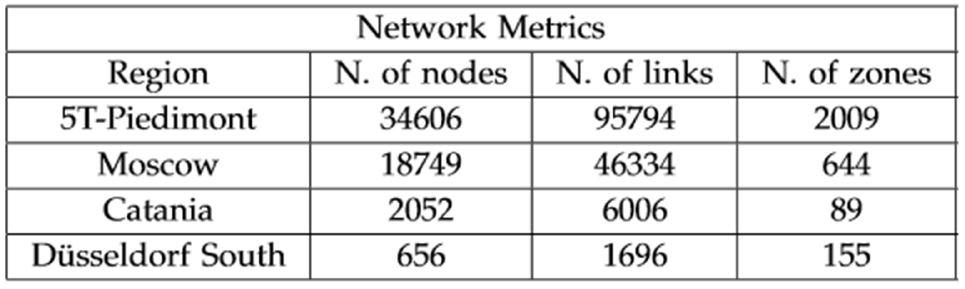
\includegraphics[width=0.7\textwidth]{PIX/netmetrics.jpg}
\end{center}
\end{table}

The tests considered the execution times of the two main (and most time-consuming) phases of the Dynamic Traffic Assignment algorithm used in the present application, namely the demand routing using \emph{Dynamic Path Search} and the \emph{Dynamic Network Loading}, i.e. the traffic propagation using the General Link Transmission Model. It should be noted that the Dynamic Path Search complexity increases with the number of arcs but the overall cost of the path search phase is mainly affected by the number of O-D \emph{zones}, while the Dynamic Network Loading computation time scales linearly with the number of nodes and links.

\subsubsection*{Route Choice Model}
Results for the Route Choice parallelisation are shown in Figure \ref{f:rcmres}, whence it is evident that performance gains are linear for 2 and 4 parallel threads, and that for larger networks the trend continues \emph{almost} linearly up to 16 threads, leading to computation time reductions between 80\% and 90\%.

It is worth noting that these are \emph{much} greater that what could be gained by parallelisation of the A* path search algorithm, even though the network used to obtain the results shown in Figure \ref{f:dsparal} was even larger than those in Table \ref{t:netmetrics}, totalling 1.1 Million nodes and 2.6 Million arcs over the \emph{entire} Austrian territory.

\fig{htbp}{PIX/rcmres.jpg}{f:rcmres}{Performance gains as reductions in Route Choice Model computation time against the number of parallel threads running serial A* searches. Different networks have very different sizes indicated in \ref{t:netmetrics}.}{width=0.6\textwidth}
\fig{htbp}{PIX/dsparal.jpg}{f:dsparal}{ Performance gains resulting from parallelisation of the A* path search algorithm, shown as the ratio of single/multi-thread execution times for the same batch of several thousand shortest path requests. Light data points in the background show the actual scatter of the execution times for the 8-thread A* search.}{width=0.6\textwidth}

\subsubsection*{Network Performance Model}
The results for the Dynamic Network Loading shown in Figure \ref{f:dnlres} are equally encouraging; they show how parallelisation overhead and inter-thread conflicts for this phase are slightly heavier, resulting soon in sub-linear gains for each additional thread. 

This \emph{saturation} effect is more and more relevant as the networks grow smaller, which would justify the choice of parallel single-thread TRE instances to share solution evaluation requests during optimisation over parallel-thread DNL.

\fig{htbp}{PIX/dnlres.jpg}{f:dnlres}{ Performance gains as reductions in Dynamic Network Loading execution time against the number of parallel threads extracting network nodes at each time step of the algorithm to compute flow cumulatives and perform kinematic wave propagation. Different networks have very different sizes indicated in \ref{t:netmetrics}. }{width=0.6\textwidth}